% Options for packages loaded elsewhere
\PassOptionsToPackage{unicode}{hyperref}
\PassOptionsToPackage{hyphens}{url}
%
\documentclass[
]{article}
\usepackage{amsmath,amssymb}
\usepackage{iftex}
\ifPDFTeX
  \usepackage[T1]{fontenc}
  \usepackage[utf8]{inputenc}
  \usepackage{textcomp} % provide euro and other symbols
\else % if luatex or xetex
  \usepackage{unicode-math} % this also loads fontspec
  \defaultfontfeatures{Scale=MatchLowercase}
  \defaultfontfeatures[\rmfamily]{Ligatures=TeX,Scale=1}
\fi
\usepackage{lmodern}
\ifPDFTeX\else
  % xetex/luatex font selection
\fi
% Use upquote if available, for straight quotes in verbatim environments
\IfFileExists{upquote.sty}{\usepackage{upquote}}{}
\IfFileExists{microtype.sty}{% use microtype if available
  \usepackage[]{microtype}
  \UseMicrotypeSet[protrusion]{basicmath} % disable protrusion for tt fonts
}{}
\makeatletter
\@ifundefined{KOMAClassName}{% if non-KOMA class
  \IfFileExists{parskip.sty}{%
    \usepackage{parskip}
  }{% else
    \setlength{\parindent}{0pt}
    \setlength{\parskip}{6pt plus 2pt minus 1pt}}
}{% if KOMA class
  \KOMAoptions{parskip=half}}
\makeatother
\usepackage{xcolor}
\usepackage[margin=1in]{geometry}
\usepackage{color}
\usepackage{fancyvrb}
\newcommand{\VerbBar}{|}
\newcommand{\VERB}{\Verb[commandchars=\\\{\}]}
\DefineVerbatimEnvironment{Highlighting}{Verbatim}{commandchars=\\\{\}}
% Add ',fontsize=\small' for more characters per line
\usepackage{framed}
\definecolor{shadecolor}{RGB}{248,248,248}
\newenvironment{Shaded}{\begin{snugshade}}{\end{snugshade}}
\newcommand{\AlertTok}[1]{\textcolor[rgb]{0.94,0.16,0.16}{#1}}
\newcommand{\AnnotationTok}[1]{\textcolor[rgb]{0.56,0.35,0.01}{\textbf{\textit{#1}}}}
\newcommand{\AttributeTok}[1]{\textcolor[rgb]{0.13,0.29,0.53}{#1}}
\newcommand{\BaseNTok}[1]{\textcolor[rgb]{0.00,0.00,0.81}{#1}}
\newcommand{\BuiltInTok}[1]{#1}
\newcommand{\CharTok}[1]{\textcolor[rgb]{0.31,0.60,0.02}{#1}}
\newcommand{\CommentTok}[1]{\textcolor[rgb]{0.56,0.35,0.01}{\textit{#1}}}
\newcommand{\CommentVarTok}[1]{\textcolor[rgb]{0.56,0.35,0.01}{\textbf{\textit{#1}}}}
\newcommand{\ConstantTok}[1]{\textcolor[rgb]{0.56,0.35,0.01}{#1}}
\newcommand{\ControlFlowTok}[1]{\textcolor[rgb]{0.13,0.29,0.53}{\textbf{#1}}}
\newcommand{\DataTypeTok}[1]{\textcolor[rgb]{0.13,0.29,0.53}{#1}}
\newcommand{\DecValTok}[1]{\textcolor[rgb]{0.00,0.00,0.81}{#1}}
\newcommand{\DocumentationTok}[1]{\textcolor[rgb]{0.56,0.35,0.01}{\textbf{\textit{#1}}}}
\newcommand{\ErrorTok}[1]{\textcolor[rgb]{0.64,0.00,0.00}{\textbf{#1}}}
\newcommand{\ExtensionTok}[1]{#1}
\newcommand{\FloatTok}[1]{\textcolor[rgb]{0.00,0.00,0.81}{#1}}
\newcommand{\FunctionTok}[1]{\textcolor[rgb]{0.13,0.29,0.53}{\textbf{#1}}}
\newcommand{\ImportTok}[1]{#1}
\newcommand{\InformationTok}[1]{\textcolor[rgb]{0.56,0.35,0.01}{\textbf{\textit{#1}}}}
\newcommand{\KeywordTok}[1]{\textcolor[rgb]{0.13,0.29,0.53}{\textbf{#1}}}
\newcommand{\NormalTok}[1]{#1}
\newcommand{\OperatorTok}[1]{\textcolor[rgb]{0.81,0.36,0.00}{\textbf{#1}}}
\newcommand{\OtherTok}[1]{\textcolor[rgb]{0.56,0.35,0.01}{#1}}
\newcommand{\PreprocessorTok}[1]{\textcolor[rgb]{0.56,0.35,0.01}{\textit{#1}}}
\newcommand{\RegionMarkerTok}[1]{#1}
\newcommand{\SpecialCharTok}[1]{\textcolor[rgb]{0.81,0.36,0.00}{\textbf{#1}}}
\newcommand{\SpecialStringTok}[1]{\textcolor[rgb]{0.31,0.60,0.02}{#1}}
\newcommand{\StringTok}[1]{\textcolor[rgb]{0.31,0.60,0.02}{#1}}
\newcommand{\VariableTok}[1]{\textcolor[rgb]{0.00,0.00,0.00}{#1}}
\newcommand{\VerbatimStringTok}[1]{\textcolor[rgb]{0.31,0.60,0.02}{#1}}
\newcommand{\WarningTok}[1]{\textcolor[rgb]{0.56,0.35,0.01}{\textbf{\textit{#1}}}}
\usepackage{graphicx}
\makeatletter
\def\maxwidth{\ifdim\Gin@nat@width>\linewidth\linewidth\else\Gin@nat@width\fi}
\def\maxheight{\ifdim\Gin@nat@height>\textheight\textheight\else\Gin@nat@height\fi}
\makeatother
% Scale images if necessary, so that they will not overflow the page
% margins by default, and it is still possible to overwrite the defaults
% using explicit options in \includegraphics[width, height, ...]{}
\setkeys{Gin}{width=\maxwidth,height=\maxheight,keepaspectratio}
% Set default figure placement to htbp
\makeatletter
\def\fps@figure{htbp}
\makeatother
\setlength{\emergencystretch}{3em} % prevent overfull lines
\providecommand{\tightlist}{%
  \setlength{\itemsep}{0pt}\setlength{\parskip}{0pt}}
\setcounter{secnumdepth}{-\maxdimen} % remove section numbering
\ifLuaTeX
  \usepackage{selnolig}  % disable illegal ligatures
\fi
\usepackage{bookmark}
\IfFileExists{xurl.sty}{\usepackage{xurl}}{} % add URL line breaks if available
\urlstyle{same}
\hypersetup{
  pdftitle={Predicting Max Attack for Arknights Operators},
  pdfauthor={Chuyu Zhuang},
  hidelinks,
  pdfcreator={LaTeX via pandoc}}

\title{Predicting Max Attack for Arknights Operators}
\author{Chuyu Zhuang}
\date{2024-09-15}

\begin{document}
\maketitle

{
\setcounter{tocdepth}{2}
\tableofcontents
}
\section{Introduction}\label{introduction}

··· \#\# Dataset Description ··· \#\# Research Questions ··· \#
Exploratory Data Analysis ··· \# Data Splitting and Cross Validation ···
\# Model Fitting and Results ··· \#\# Linear Regression \ldots{} \#\#
Lasso Regression \ldots{} \#\# Random Forest ··· \# Model Selection and
Performance \ldots{} \#\# Linear Regression Coefficients \ldots{} \#\#
Lasso Regression Coefficients \ldots{} \#\# Random Forest Variable
Importance ··· \# Conclusion ···

\section{1. Introduction}\label{introduction-1}

This is a model that predicts the maximum attack power of arknights
operators.

\subsection{What is Arknights?}\label{what-is-arknights}

``Arknights'' is a strategy tower defense mobile game developed by
Hypergryph Network, and it is also the first game developed by
Hypergryph Network.You can think of it as a anime version of Plants
vs.~Zombies, except that the plants here are employees working in your
company, and the one who tells you to work is not Crazy Dave but a green
old lynx who likes to tell
riddles.\includegraphics{"C:/Users/zhuan/Downloads/131final/立绘_凯尔希_1.png"}

\subsection{What are we doing?}\label{what-are-we-doing}

This project focuses on predicting the \textbf{max attack} of new
operators based on existing data, particularly by linking the operator's
class, stars, and Initial deployment cost with their maximum attack.

\subsection{Why?}\label{why}

Like many gacha games, Arknights regularly releases new characters
(referred to as operators in the game). In the past, players mostly
decided whether to pull for a character based on the quality of their
artwork or their portrayal in the storyline. However, as the game has
continued to update and increase in difficulty, players have gradually
started to decide whether to pull for new operators based on their
strength.

\section{2. Exploratory Data Analysis}\label{exploratory-data-analysis}

First, we will load all of our packages and the raw data, followed by
performing exploratory analysis to understand the relationships between
key variables and the response variable, \textbf{max attack}. from
Kaggle\href{https://www.kaggle.com/datasets/victorsoeiro/arknights-operators/data}{this
link}

\begin{Shaded}
\begin{Highlighting}[]
\CommentTok{\# Load necessary libraries}
\FunctionTok{library}\NormalTok{(ggplot2)}
\FunctionTok{library}\NormalTok{(readr)}
\FunctionTok{library}\NormalTok{(dplyr)}
\end{Highlighting}
\end{Shaded}

\begin{verbatim}
## 
## 载入程序包:'dplyr'
\end{verbatim}

\begin{verbatim}
## The following objects are masked from 'package:stats':
## 
##     filter, lag
\end{verbatim}

\begin{verbatim}
## The following objects are masked from 'package:base':
## 
##     intersect, setdiff, setequal, union
\end{verbatim}

\begin{Shaded}
\begin{Highlighting}[]
\FunctionTok{library}\NormalTok{(car)}
\end{Highlighting}
\end{Shaded}

\begin{verbatim}
## 载入需要的程序包:carData
\end{verbatim}

\begin{verbatim}
## 
## 载入程序包:'car'
\end{verbatim}

\begin{verbatim}
## The following object is masked from 'package:dplyr':
## 
##     recode
\end{verbatim}

\begin{Shaded}
\begin{Highlighting}[]
\FunctionTok{library}\NormalTok{(MASS)}
\end{Highlighting}
\end{Shaded}

\begin{verbatim}
## 
## 载入程序包:'MASS'
\end{verbatim}

\begin{verbatim}
## The following object is masked from 'package:dplyr':
## 
##     select
\end{verbatim}

\begin{Shaded}
\begin{Highlighting}[]
\FunctionTok{library}\NormalTok{(caret)}
\end{Highlighting}
\end{Shaded}

\begin{verbatim}
## 载入需要的程序包:lattice
\end{verbatim}

\begin{Shaded}
\begin{Highlighting}[]
\FunctionTok{library}\NormalTok{(e1071)}
\FunctionTok{library}\NormalTok{(xgboost)}
\end{Highlighting}
\end{Shaded}

\begin{verbatim}
## 
## 载入程序包:'xgboost'
\end{verbatim}

\begin{verbatim}
## The following object is masked from 'package:dplyr':
## 
##     slice
\end{verbatim}

\begin{Shaded}
\begin{Highlighting}[]
\FunctionTok{library}\NormalTok{(rsample)}
\end{Highlighting}
\end{Shaded}

\begin{verbatim}
## 
## 载入程序包:'rsample'
\end{verbatim}

\begin{verbatim}
## The following object is masked from 'package:e1071':
## 
##     permutations
\end{verbatim}

\begin{Shaded}
\begin{Highlighting}[]
\CommentTok{\# Load the dataset}
\NormalTok{data }\OtherTok{\textless{}{-}} \FunctionTok{read\_csv}\NormalTok{(}\StringTok{"data.csv"}\NormalTok{)}
\end{Highlighting}
\end{Shaded}

\begin{verbatim}
## Rows: 235 Columns: 63
## -- Column specification --------------------------------------------------------
## Delimiter: ","
## chr (44): name, class, branch, faction, stars, position, tags, trait, availa...
## dbl (19): base_hp, elite_1_hp, trust_hp, base_atk, elite_1_atk, trust_atk, b...
## 
## i Use `spec()` to retrieve the full column specification for this data.
## i Specify the column types or set `show_col_types = FALSE` to quiet this message.
\end{verbatim}

\begin{Shaded}
\begin{Highlighting}[]
\CommentTok{\# Display first few rows of the dataset}
\FunctionTok{head}\NormalTok{(data)}
\end{Highlighting}
\end{Shaded}

\begin{verbatim}
## # A tibble: 6 x 63
##   name        class branch faction stars position tags  trait availability icon 
##   <chr>       <chr> <chr>  <chr>   <chr> <chr>    <chr> <chr> <chr>        <chr>
## 1 "Castle-3"  Guard Dread~ Rhodes~ 1-st~ Melee    ['Su~ Bloc~ Recruitment  http~
## 2 "\"Justice~ Snip~ Marks~ Pinus ~ 1-st~ Ranged   ['Su~ Atta~ Recruitment  http~
## 3 "Lancet-2"  Medic Medic  Rhodes~ 1-st~ Ranged   ['He~ Rest~ Recruitment~ http~
## 4 "THRM-EX"   Spec~ Execu~ Rhodes~ 1-st~ Melee    ['Nu~ Does~ Recruitment~ http~
## 5 "12F"       Cast~ Splash Rhodes~ 2-st~ Ranged   ['St~ Deal~ Recruitment~ http~
## 6 "Durin"     Cast~ Core   Rhodes~ 2-st~ Ranged   ['St~ Deal~ Recruitment~ http~
## # i 53 more variables: description <chr>, phrase <chr>, file_no. <chr>,
## #   gender <chr>, height <chr>, mobility <chr>, endurance <chr>,
## #   internal_name <chr>, base_hp <dbl>, elite_1_hp <dbl>, elite_2_hp <chr>,
## #   max_hp <chr>, trust_hp <dbl>, base_atk <dbl>, elite_1_atk <dbl>,
## #   elite_2_atk <chr>, max_atk <chr>, trust_atk <dbl>, base_def <dbl>,
## #   elite_1_def <dbl>, elite_2_def <chr>, max_def <chr>, trust_def <dbl>,
## #   base_res <dbl>, elite_1_res <dbl>, elite_2_res <chr>, max_res <chr>, ...
\end{verbatim}

\subsection{Variable Selection}\label{variable-selection}

Let's mess around with the data a little bit to see what we're currently
working with

\begin{Shaded}
\begin{Highlighting}[]
\FunctionTok{dim}\NormalTok{(data)}
\end{Highlighting}
\end{Shaded}

\begin{verbatim}
## [1] 235  63
\end{verbatim}

We can see that the entire data has 235 rows and 63 columns, which means
there are 235 operators and 63 columns of variables. However, from the
data, variables such as faction, tags, trait, availability, icon,
description, phrase, file\_no and other game-related variables are
insignificant to the analysis of the maximum attack power of operators
(after all, in this game, even if you only hold a water gun in the plot,
you can become a super powerful operator in terms of strength).So we can
ignore these irrelevant variables.

Some people may notice that there is a variable called branch after
class. This is a category created by the game to subdivide different
operators in the same class. Let's see how many branches there are in
total.

\begin{Shaded}
\begin{Highlighting}[]
\NormalTok{distinct\_count }\OtherTok{\textless{}{-}}\NormalTok{ data }\SpecialCharTok{\%\textgreater{}\%}
  \FunctionTok{summarise}\NormalTok{(}\AttributeTok{n\_distinct =} \FunctionTok{n\_distinct}\NormalTok{(branch))}

\FunctionTok{print}\NormalTok{(distinct\_count)}
\end{Highlighting}
\end{Shaded}

\begin{verbatim}
## # A tibble: 1 x 1
##   n_distinct
##        <int>
## 1         52
\end{verbatim}

There are 253 operators in total but there are 53 branches, which means
that each branch has only 4-5 operators on average. In actual
situations, some branches only have 2-3 operators. For this reason, we
can also ignore this variable and focus on the class variable.

Similarly, since our goal is to focus on the maximum attack power of the
operator, something like
base\_hp,elite\_1\_hp,elite\_2\_hp,max\_hp,trust\_hp,base\_atk,elite\_1\_atk,elite\_2\_atk,trust\_atk,base\_def,elite\_1\_def,elite\_2\_def,max\_def,trust\_def,base\_res,elite\_1\_res,elite\_2\_res,max\_res,base\_redeploy,elite\_1\_redeploy,elite\_2\_redeploy,max\_redeploy,base\_dp\_cost,e
lite\_1\_dp\_cost,elite\_2\_dp\_cost,max\_dp\_cost,base\_block,elite\_1\_block,elite\_2\_block,max\_block,base\_interval,elite\_1\_interval,elite\_2\_interval,max\_interval,images,experience,place\_of\_birth,date\_of\_birth,race,infection\_status,strength,tactical\_acumen,combat\_skill,arts\_ada
ptability variables can be omitted

Now, let's filter out all those unwanted variables and our dataset will
be ready for further tidying

\begin{Shaded}
\begin{Highlighting}[]
\NormalTok{data }\OtherTok{\textless{}{-}}\NormalTok{ data }\SpecialCharTok{\%\textgreater{}\%}
\NormalTok{  dplyr}\SpecialCharTok{::}\FunctionTok{select}\NormalTok{(}\StringTok{"name"}\NormalTok{,}\StringTok{"class"}\NormalTok{, }\StringTok{"stars"}\NormalTok{, }\StringTok{"position"}\NormalTok{, }\StringTok{"max\_atk"}\NormalTok{)}
\end{Highlighting}
\end{Shaded}

\subsubsection{Missing data review and
cleaning}\label{missing-data-review-and-cleaning}

Next, let's see if there is any missing data.

\begin{Shaded}
\begin{Highlighting}[]
\CommentTok{\# View non{-}numeric max\_atk data}
\NormalTok{non\_numeric\_values }\OtherTok{\textless{}{-}}\NormalTok{ data[}\FunctionTok{is.na}\NormalTok{(}\FunctionTok{as.numeric}\NormalTok{(}\FunctionTok{as.character}\NormalTok{(data}\SpecialCharTok{$}\NormalTok{max\_atk))), ]}
\end{Highlighting}
\end{Shaded}

\begin{verbatim}
## Warning in `[.tbl_df`(data, is.na(as.numeric(as.character(data$max_atk))), :
## 强制改变过程中产生了NA
\end{verbatim}

\begin{Shaded}
\begin{Highlighting}[]
\CommentTok{\# Print rows with non{-}numeric max\_atk (process as needed)}
\FunctionTok{print}\NormalTok{(non\_numeric\_values)}
\end{Highlighting}
\end{Shaded}

\begin{verbatim}
## # A tibble: 26 x 5
##    name                 class      stars  position max_atk
##    <chr>                <chr>      <chr>  <chr>    <chr>  
##  1 "Castle-3"           Guard      1-star Melee    –      
##  2 "\"Justice Knight\"" Sniper     1-star Ranged   –      
##  3 "Lancet-2"           Medic      1-star Ranged   –      
##  4 "THRM-EX"            Specialist 1-star Melee    –      
##  5 "12F"                Caster     2-star Ranged   –      
##  6 "Durin"              Caster     2-star Ranged   –      
##  7 "Noir Corne"         Defender   2-star Melee    –      
##  8 "Rangers"            Sniper     2-star Ranged   –      
##  9 "Yato"               Vanguard   2-star Melee    –      
## 10 "Adnachiel"          Sniper     3-star Ranged   –      
## # i 16 more rows
\end{verbatim}

We can see that operators below 3 stars do not have the highest attack
power, Because they cannot be upgraded to Elite Level 2, we need to
clear them as missing data

\begin{Shaded}
\begin{Highlighting}[]
\CommentTok{\# Force max\_atk to numeric and process NAs}
\NormalTok{data}\SpecialCharTok{$}\NormalTok{max\_atk }\OtherTok{\textless{}{-}} \FunctionTok{as.numeric}\NormalTok{(}\FunctionTok{as.character}\NormalTok{(data}\SpecialCharTok{$}\NormalTok{max\_atk))}

\CommentTok{\# Remove rows with NA values}
\NormalTok{data\_clean }\OtherTok{\textless{}{-}}\NormalTok{ data[}\SpecialCharTok{!}\FunctionTok{is.na}\NormalTok{(data}\SpecialCharTok{$}\NormalTok{max\_atk), ]}

\FunctionTok{print}\NormalTok{(data\_clean)}
\end{Highlighting}
\end{Shaded}

\begin{verbatim}
## # A tibble: 209 x 5
##    name       class    stars  position max_atk
##    <chr>      <chr>    <chr>  <chr>      <dbl>
##  1 Aciddrop   Sniper   4-star Ranged       735
##  2 Ambriel    Sniper   4-star Ranged       977
##  3 Arene      Guard    4-star Melee        640
##  4 Beanstalk  Vanguard 4-star Ranged       405
##  5 Beehunter  Guard    4-star Melee        513
##  6 Bubble     Defender 4-star Melee        370
##  7 Chestnut   Medic    4-star Ranged       389
##  8 Click      Caster   4-star Ranged       315
##  9 Conviction Guard    4-star Melee        929
## 10 Courier    Vanguard 4-star Melee        435
## # i 199 more rows
\end{verbatim}

\subsubsection{Univariate Analysis: Distribution of Max
Attack}\label{univariate-analysis-distribution-of-max-attack}

First, let's look at the distribution of maximum attack power.

\begin{Shaded}
\begin{Highlighting}[]
\CommentTok{\# Plotting the distribution of max attack}
\FunctionTok{ggplot}\NormalTok{(data\_clean, }\FunctionTok{aes}\NormalTok{(}\AttributeTok{x =}\NormalTok{ max\_atk)) }\SpecialCharTok{+}
  \FunctionTok{geom\_histogram}\NormalTok{(}\AttributeTok{binwidth =} \DecValTok{50}\NormalTok{, }\AttributeTok{fill =} \StringTok{"blue"}\NormalTok{, }\AttributeTok{color =} \StringTok{"white"}\NormalTok{) }\SpecialCharTok{+}
  \FunctionTok{labs}\NormalTok{(}\AttributeTok{title =} \StringTok{"Distribution of Base Attack"}\NormalTok{, }\AttributeTok{x =} \StringTok{"Base Attack"}\NormalTok{, }\AttributeTok{y =} \StringTok{"Count"}\NormalTok{)}
\end{Highlighting}
\end{Shaded}

\includegraphics{Updated_Arknights_Operators_Project_Report_files/figure-latex/unnamed-chunk-8-1.pdf}

\paragraph{What can we find?}\label{what-can-we-find}

\begin{itemize}
\tightlist
\item
  The distribution of max attack shows that the maximum attack power of
  550 operators is the most, with fewer operators having extremely high
  or low values.
\end{itemize}

\subsubsection{Bivariate Analysis: Relationship Between Predictors and
Max
Attack}\label{bivariate-analysis-relationship-between-predictors-and-max-attack}

Next, let's look at the relationship between the star and position and
the maximum attack power.

\begin{Shaded}
\begin{Highlighting}[]
\CommentTok{\# Plotting relationships between class, stars, and max attack}
\FunctionTok{ggplot}\NormalTok{(data\_clean, }\FunctionTok{aes}\NormalTok{(}\AttributeTok{x =}\NormalTok{ class, }\AttributeTok{y =}\NormalTok{ max\_atk, }\AttributeTok{fill =}\NormalTok{ stars)) }\SpecialCharTok{+} 
  \FunctionTok{geom\_boxplot}\NormalTok{() }\SpecialCharTok{+} 
  \FunctionTok{ggtitle}\NormalTok{(}\StringTok{"Max Attack Distribution by Class and stars"}\NormalTok{)}
\end{Highlighting}
\end{Shaded}

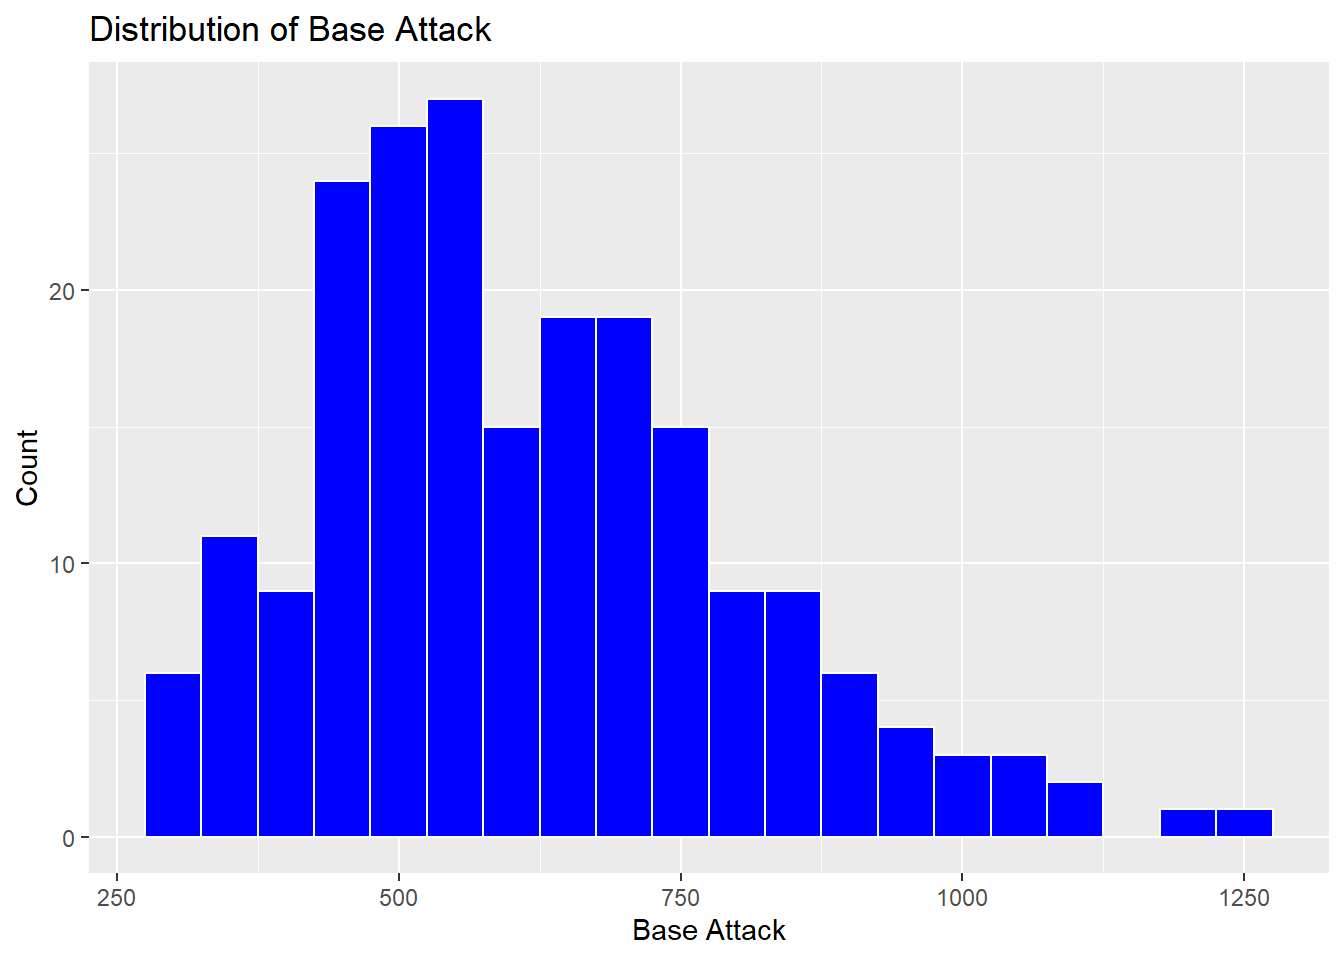
\includegraphics{Updated_Arknights_Operators_Project_Report_files/figure-latex/unnamed-chunk-9-1.pdf}

\begin{Shaded}
\begin{Highlighting}[]
\CommentTok{\# Plotting relationships between class, positions, and max attack}
\FunctionTok{ggplot}\NormalTok{(data\_clean, }\FunctionTok{aes}\NormalTok{(}\AttributeTok{x =}\NormalTok{ stars, }\AttributeTok{y =}\NormalTok{ max\_atk, }\AttributeTok{color =}\NormalTok{ position)) }\SpecialCharTok{+}
  \FunctionTok{geom\_boxplot}\NormalTok{() }\SpecialCharTok{+}
  \FunctionTok{labs}\NormalTok{(}\AttributeTok{title =} \StringTok{"Max Attack by Stars and Position"}\NormalTok{, }\AttributeTok{x =} \StringTok{"Stars"}\NormalTok{, }\AttributeTok{y =} \StringTok{"Max Attack"}\NormalTok{) }\SpecialCharTok{+}
  \FunctionTok{theme\_minimal}\NormalTok{()}
\end{Highlighting}
\end{Shaded}

\includegraphics{Updated_Arknights_Operators_Project_Report_files/figure-latex/unnamed-chunk-9-2.pdf}

\paragraph{What can we find?}\label{what-can-we-find-1}

\begin{itemize}
\tightlist
\item
  Operators with higher stars and certain classes tend to have higher
  max attack values, as shown by the spread in the box plots.
\end{itemize}

-Regardless of the star level, the maximum value of the ranged attack
power is higher than the maximum value of the melee, but the minimum
value is lower than the minimum value of the melee.

\section{3. Data Splitting and Cross
Validation}\label{data-splitting-and-cross-validation}

The first step we must take before fitting any model is to split our
data into a training set and a test set. The training set will be used
to do just that: train our model. The test set acts as a test because
our model will not be trained using this data. Therefore, once we fit
what we consider to be the ``best'' model (usually based on the lowest
RMSE, or Root Mean Squared Error of regression) to our test set, we will
see how it truly performs on new data. By splitting our data into a test
set and a training set, we can avoid overfitting because the model is
not learning using all of the available data. The split that I chose is
a 70/30 split, meaning that 70\% of the data will go into the training
set and 30\% of the data will go into the test set. This way, the
majority of our data is used to train the model; however, we still have
enough data to test the model. Additionally, the split is stratified
based on the outcome variable, max\_atk, to ensure that the max\_atk
distributions for the training and test data are equal.

\begin{Shaded}
\begin{Highlighting}[]
\CommentTok{\# Data Splitting}
\FunctionTok{set.seed}\NormalTok{(}\DecValTok{123}\NormalTok{)}
\NormalTok{data\_split }\OtherTok{\textless{}{-}} \FunctionTok{initial\_split}\NormalTok{(data\_clean, }\AttributeTok{prop =} \FloatTok{0.7}\NormalTok{, }\AttributeTok{strata =}\NormalTok{ max\_atk)}
\NormalTok{train }\OtherTok{\textless{}{-}} \FunctionTok{training}\NormalTok{(data\_split)}
\NormalTok{test }\OtherTok{\textless{}{-}} \FunctionTok{testing}\NormalTok{(data\_split)}

\CommentTok{\# Define cross validation controls}
\NormalTok{ctrl }\OtherTok{\textless{}{-}} \FunctionTok{trainControl}\NormalTok{(}\AttributeTok{method =} \StringTok{"cv"}\NormalTok{, }\AttributeTok{number =} \DecValTok{10}\NormalTok{)}
\end{Highlighting}
\end{Shaded}

check the data split correct

\begin{Shaded}
\begin{Highlighting}[]
\FunctionTok{nrow}\NormalTok{(train)}\SpecialCharTok{/}\FunctionTok{nrow}\NormalTok{(data\_clean)}
\end{Highlighting}
\end{Shaded}

\begin{verbatim}
## [1] 0.6937799
\end{verbatim}

\begin{Shaded}
\begin{Highlighting}[]
\FunctionTok{nrow}\NormalTok{(test)}\SpecialCharTok{/}\FunctionTok{nrow}\NormalTok{(train)}
\end{Highlighting}
\end{Shaded}

\begin{verbatim}
## [1] 0.4413793
\end{verbatim}

The training set has about 70\% of the data and the testing set has
about 30\% of the data. So, the data was split correctly between the
training and testing sets.

\section{4. Model Fitting and Results}\label{model-fitting-and-results}

We will now build several machine learning models to predict the
\textbf{max attack} of new operators.

\subsubsection{Model 1: linear regression
model}\label{model-1-linear-regression-model}

\begin{Shaded}
\begin{Highlighting}[]
\CommentTok{\# Fit a linear regression model using class, stars, and Initial deployment cost as predictors}
\NormalTok{model\_lm }\OtherTok{\textless{}{-}} \FunctionTok{train}\NormalTok{(max\_atk }\SpecialCharTok{\textasciitilde{}}\NormalTok{ class }\SpecialCharTok{+}\NormalTok{ stars }\SpecialCharTok{+}\NormalTok{ position, }
                  \AttributeTok{data =}\NormalTok{ train, }
                  \AttributeTok{method =} \StringTok{"lm"}\NormalTok{, }
                  \AttributeTok{trControl =}\NormalTok{ ctrl)}

\CommentTok{\# Summary of the linear model}
\FunctionTok{summary}\NormalTok{(model\_lm}\SpecialCharTok{$}\NormalTok{finalModel)}
\end{Highlighting}
\end{Shaded}

\begin{verbatim}
## 
## Call:
## lm(formula = .outcome ~ ., data = dat)
## 
## Residuals:
##     Min      1Q  Median      3Q     Max 
## -402.60  -86.11   -8.76   63.95  491.68 
## 
## Coefficients:
##                 Estimate Std. Error t value Pr(>|t|)    
## (Intercept)       746.97      87.38   8.549 2.47e-14 ***
## classDefender    -190.42      95.18  -2.001  0.04746 *  
## classGuard        -89.05      91.24  -0.976  0.33079    
## classMedic       -235.76      53.54  -4.404 2.16e-05 ***
## classSniper        12.39      46.74   0.265  0.79130    
## classSpecialist  -130.25      89.89  -1.449  0.14967    
## classSupporter   -246.94      50.27  -4.912 2.58e-06 ***
## classVanguard    -261.06      90.62  -2.881  0.00462 ** 
## `stars5-star`      43.74      31.92   1.370  0.17290    
## `stars6-star`     109.28      35.89   3.045  0.00280 ** 
## positionRanged   -122.65      79.94  -1.534  0.12734    
## ---
## Signif. codes:  0 '***' 0.001 '**' 0.01 '*' 0.05 '.' 0.1 ' ' 1
## 
## Residual standard error: 151.4 on 134 degrees of freedom
## Multiple R-squared:  0.3625, Adjusted R-squared:  0.3149 
## F-statistic: 7.619 on 10 and 134 DF,  p-value: 1.484e-09
\end{verbatim}

\subsubsection{Model 2: Lasso
regression}\label{model-2-lasso-regression}

\begin{Shaded}
\begin{Highlighting}[]
\CommentTok{\# Train Lasso regression model with the adjusted predictors}
\NormalTok{model\_lasso }\OtherTok{\textless{}{-}} \FunctionTok{train}\NormalTok{(max\_atk }\SpecialCharTok{\textasciitilde{}}\NormalTok{ class }\SpecialCharTok{+}\NormalTok{ stars }\SpecialCharTok{+}\NormalTok{ position,}
                     \AttributeTok{data =}\NormalTok{ train,}
                     \AttributeTok{method =} \StringTok{"glmnet"}\NormalTok{,}
                     \AttributeTok{trControl =}\NormalTok{ ctrl,}
                     \AttributeTok{tuneLength =} \DecValTok{5}\NormalTok{)}

\CommentTok{\# Print Lasso model summary}
\FunctionTok{print}\NormalTok{(model\_lasso)}
\end{Highlighting}
\end{Shaded}

\begin{verbatim}
## glmnet 
## 
## 145 samples
##   3 predictor
## 
## No pre-processing
## Resampling: Cross-Validated (10 fold) 
## Summary of sample sizes: 129, 131, 130, 130, 132, 132, ... 
## Resampling results across tuning parameters:
## 
##   alpha  lambda       RMSE      Rsquared   MAE     
##   0.100   0.05669914  149.7943  0.3504850  115.0645
##   0.100   0.26317410  149.7600  0.3505127  115.0319
##   0.100   1.22154598  149.6407  0.3495121  115.0451
##   0.100   5.66991419  149.6303  0.3450433  115.4381
##   0.100  26.31741040  150.3043  0.3382401  115.8907
##   0.325   0.05669914  149.7914  0.3505947  115.0689
##   0.325   0.26317410  149.7342  0.3504401  115.0062
##   0.325   1.22154598  149.6426  0.3483420  115.1778
##   0.325   5.66991419  150.0261  0.3385029  116.0554
##   0.325  26.31741040  150.5969  0.3402859  116.0283
##   0.550   0.05669914  149.7886  0.3505542  115.0665
##   0.550   0.26317410  149.7112  0.3503475  114.9856
##   0.550   1.22154598  149.6931  0.3466456  115.4270
##   0.550   5.66991419  149.8371  0.3385849  115.8370
##   0.550  26.31741040  151.6822  0.3423615  116.5939
##   0.775   0.05669914  149.7888  0.3505896  115.0679
##   0.775   0.26317410  149.6910  0.3502323  114.9849
##   0.775   1.22154598  149.6659  0.3457411  115.6037
##   0.775   5.66991419  149.6352  0.3399255  115.6232
##   0.775  26.31741040  154.2923  0.3333257  119.3771
##   1.000   0.05669914  149.7809  0.3506140  115.0599
##   1.000   0.26317410  149.6749  0.3500780  115.0087
##   1.000   1.22154598  149.5358  0.3463678  115.5118
##   1.000   5.66991419  149.5242  0.3411336  115.4730
##   1.000  26.31741040  157.8825  0.3155988  124.0377
## 
## RMSE was used to select the optimal model using the smallest value.
## The final values used for the model were alpha = 1 and lambda = 5.669914.
\end{verbatim}

\subsubsection{Model 3: Random forest
model}\label{model-3-random-forest-model}

\begin{Shaded}
\begin{Highlighting}[]
\CommentTok{\# Train Lasso regression model with the adjusted predictors}
\NormalTok{model\_rf }\OtherTok{\textless{}{-}} \FunctionTok{train}\NormalTok{(max\_atk }\SpecialCharTok{\textasciitilde{}}\NormalTok{ class }\SpecialCharTok{+}\NormalTok{ stars }\SpecialCharTok{+}\NormalTok{ position,}
                  \AttributeTok{data =}\NormalTok{ train,}
                  \AttributeTok{method =} \StringTok{"rf"}\NormalTok{,}
                  \AttributeTok{trControl =}\NormalTok{ ctrl,}
                  \AttributeTok{tuneLength =} \DecValTok{5}\NormalTok{)}


\CommentTok{\# Print Lasso model summary}
\FunctionTok{print}\NormalTok{(model\_lasso)}
\end{Highlighting}
\end{Shaded}

\begin{verbatim}
## glmnet 
## 
## 145 samples
##   3 predictor
## 
## No pre-processing
## Resampling: Cross-Validated (10 fold) 
## Summary of sample sizes: 129, 131, 130, 130, 132, 132, ... 
## Resampling results across tuning parameters:
## 
##   alpha  lambda       RMSE      Rsquared   MAE     
##   0.100   0.05669914  149.7943  0.3504850  115.0645
##   0.100   0.26317410  149.7600  0.3505127  115.0319
##   0.100   1.22154598  149.6407  0.3495121  115.0451
##   0.100   5.66991419  149.6303  0.3450433  115.4381
##   0.100  26.31741040  150.3043  0.3382401  115.8907
##   0.325   0.05669914  149.7914  0.3505947  115.0689
##   0.325   0.26317410  149.7342  0.3504401  115.0062
##   0.325   1.22154598  149.6426  0.3483420  115.1778
##   0.325   5.66991419  150.0261  0.3385029  116.0554
##   0.325  26.31741040  150.5969  0.3402859  116.0283
##   0.550   0.05669914  149.7886  0.3505542  115.0665
##   0.550   0.26317410  149.7112  0.3503475  114.9856
##   0.550   1.22154598  149.6931  0.3466456  115.4270
##   0.550   5.66991419  149.8371  0.3385849  115.8370
##   0.550  26.31741040  151.6822  0.3423615  116.5939
##   0.775   0.05669914  149.7888  0.3505896  115.0679
##   0.775   0.26317410  149.6910  0.3502323  114.9849
##   0.775   1.22154598  149.6659  0.3457411  115.6037
##   0.775   5.66991419  149.6352  0.3399255  115.6232
##   0.775  26.31741040  154.2923  0.3333257  119.3771
##   1.000   0.05669914  149.7809  0.3506140  115.0599
##   1.000   0.26317410  149.6749  0.3500780  115.0087
##   1.000   1.22154598  149.5358  0.3463678  115.5118
##   1.000   5.66991419  149.5242  0.3411336  115.4730
##   1.000  26.31741040  157.8825  0.3155988  124.0377
## 
## RMSE was used to select the optimal model using the smallest value.
## The final values used for the model were alpha = 1 and lambda = 5.669914.
\end{verbatim}

\section{5. Model Selection and
Performance}\label{model-selection-and-performance}

We compare the performance of the models based on RMSE, and select the
best-performing model.

\begin{Shaded}
\begin{Highlighting}[]
\CommentTok{\# Predict on test set}
\NormalTok{pred\_lm }\OtherTok{\textless{}{-}} \FunctionTok{predict}\NormalTok{(model\_lm, }\AttributeTok{newdata =}\NormalTok{ test)}
\NormalTok{pred\_lasso }\OtherTok{\textless{}{-}} \FunctionTok{predict}\NormalTok{(model\_lasso, }\AttributeTok{newdata =}\NormalTok{ test)}
\NormalTok{pred\_rf }\OtherTok{\textless{}{-}} \FunctionTok{predict}\NormalTok{(model\_rf, }\AttributeTok{newdata =}\NormalTok{ test)}

\CommentTok{\# Calculate RMSE for each model}
\NormalTok{rmse\_lm }\OtherTok{\textless{}{-}} \FunctionTok{sqrt}\NormalTok{(}\FunctionTok{mean}\NormalTok{((test}\SpecialCharTok{$}\NormalTok{max\_atk }\SpecialCharTok{{-}}\NormalTok{ pred\_lm)}\SpecialCharTok{\^{}}\DecValTok{2}\NormalTok{))}
\NormalTok{rmse\_lasso }\OtherTok{\textless{}{-}} \FunctionTok{sqrt}\NormalTok{(}\FunctionTok{mean}\NormalTok{((test}\SpecialCharTok{$}\NormalTok{max\_atk }\SpecialCharTok{{-}}\NormalTok{ pred\_lasso)}\SpecialCharTok{\^{}}\DecValTok{2}\NormalTok{))}
\NormalTok{rmse\_rf }\OtherTok{\textless{}{-}} \FunctionTok{sqrt}\NormalTok{(}\FunctionTok{mean}\NormalTok{((test}\SpecialCharTok{$}\NormalTok{max\_atk }\SpecialCharTok{{-}}\NormalTok{ pred\_rf)}\SpecialCharTok{\^{}}\DecValTok{2}\NormalTok{))}

\CommentTok{\# Print RMSE results}
\FunctionTok{print}\NormalTok{(}\FunctionTok{paste}\NormalTok{(}\StringTok{"Linear Regression RMSE:"}\NormalTok{, rmse\_lm))}
\end{Highlighting}
\end{Shaded}

\begin{verbatim}
## [1] "Linear Regression RMSE: 165.035647868777"
\end{verbatim}

\begin{Shaded}
\begin{Highlighting}[]
\FunctionTok{print}\NormalTok{(}\FunctionTok{paste}\NormalTok{(}\StringTok{"Lasso Regression RMSE:"}\NormalTok{, rmse\_lasso))}
\end{Highlighting}
\end{Shaded}

\begin{verbatim}
## [1] "Lasso Regression RMSE: 168.767820416791"
\end{verbatim}

\begin{Shaded}
\begin{Highlighting}[]
\FunctionTok{print}\NormalTok{(}\FunctionTok{paste}\NormalTok{(}\StringTok{"Random Forest RMSE:"}\NormalTok{, rmse\_rf))}
\end{Highlighting}
\end{Shaded}

\begin{verbatim}
## [1] "Random Forest RMSE: 166.862616730871"
\end{verbatim}

\subsection{Linear Regression
Coefficients}\label{linear-regression-coefficients}

We visualize the coefficients for the Linear Regression model.

\begin{Shaded}
\begin{Highlighting}[]
\CommentTok{\# Extract coefficients}
\NormalTok{lm\_coefs }\OtherTok{\textless{}{-}} \FunctionTok{coef}\NormalTok{(model\_lm}\SpecialCharTok{$}\NormalTok{finalModel)}

\CommentTok{\# Create a data frame for visualization}
\NormalTok{coef\_df }\OtherTok{\textless{}{-}} \FunctionTok{data.frame}\NormalTok{(}
  \AttributeTok{Variable =} \FunctionTok{names}\NormalTok{(lm\_coefs),}
  \AttributeTok{Coefficient =}\NormalTok{ lm\_coefs}
\NormalTok{)}

\CommentTok{\# Plot coefficients}
\FunctionTok{ggplot}\NormalTok{(coef\_df, }\FunctionTok{aes}\NormalTok{(}\AttributeTok{x =}\NormalTok{ Variable, }\AttributeTok{y =}\NormalTok{ Coefficient)) }\SpecialCharTok{+}
  \FunctionTok{geom\_bar}\NormalTok{(}\AttributeTok{stat =} \StringTok{"identity"}\NormalTok{) }\SpecialCharTok{+}
  \FunctionTok{ggtitle}\NormalTok{(}\StringTok{"Linear Regression Coefficients"}\NormalTok{)}
\end{Highlighting}
\end{Shaded}

\includegraphics{Updated_Arknights_Operators_Project_Report_files/figure-latex/unnamed-chunk-16-1.pdf}

\subsection{Lasso Regression
Coefficients}\label{lasso-regression-coefficients}

Similarly, we extract and visualize the coefficients for the Lasso
model.

\begin{Shaded}
\begin{Highlighting}[]
\CommentTok{\# Extract the coefficients of the Lasso regression model}
\NormalTok{lasso\_coefs }\OtherTok{\textless{}{-}} \FunctionTok{coef}\NormalTok{(model\_lasso}\SpecialCharTok{$}\NormalTok{finalModel, model\_lasso}\SpecialCharTok{$}\NormalTok{bestTune}\SpecialCharTok{$}\NormalTok{lambda)}

\CommentTok{\# Create a data frame for visualization}
\NormalTok{coef\_df\_lasso }\OtherTok{\textless{}{-}} \FunctionTok{data.frame}\NormalTok{(}
\AttributeTok{Variable =} \FunctionTok{rownames}\NormalTok{(lasso\_coefs),}
\AttributeTok{Coefficient =} \FunctionTok{as.vector}\NormalTok{(lasso\_coefs)}
\NormalTok{)}

\CommentTok{\# Plot the coefficients of the Lasso regression model}
\FunctionTok{ggplot}\NormalTok{(coef\_df\_lasso, }\FunctionTok{aes}\NormalTok{(}\AttributeTok{x =}\NormalTok{ Variable, }\AttributeTok{y =}\NormalTok{ Coefficient)) }\SpecialCharTok{+}
\FunctionTok{geom\_bar}\NormalTok{(}\AttributeTok{stat =} \StringTok{"identity"}\NormalTok{) }\SpecialCharTok{+}
\FunctionTok{ggtitle}\NormalTok{(}\StringTok{"Lasso Regression Coefficients"}\NormalTok{)}
\end{Highlighting}
\end{Shaded}

\includegraphics{Updated_Arknights_Operators_Project_Report_files/figure-latex/unnamed-chunk-17-1.pdf}

\subsection{Random Forest Variable
Importance}\label{random-forest-variable-importance}

Finally, we visualize the variable importance for the Random Forest
model.

\begin{Shaded}
\begin{Highlighting}[]
\CommentTok{\# Extract variable importance of random forest model}
\NormalTok{importance\_rf }\OtherTok{\textless{}{-}} \FunctionTok{varImp}\NormalTok{(model\_rf)}

\CommentTok{\# Draw variable importance graph of random forest model}
\FunctionTok{plot}\NormalTok{(importance\_rf, }\AttributeTok{main =} \StringTok{"Random Forest Variable Importance"}\NormalTok{)}
\end{Highlighting}
\end{Shaded}

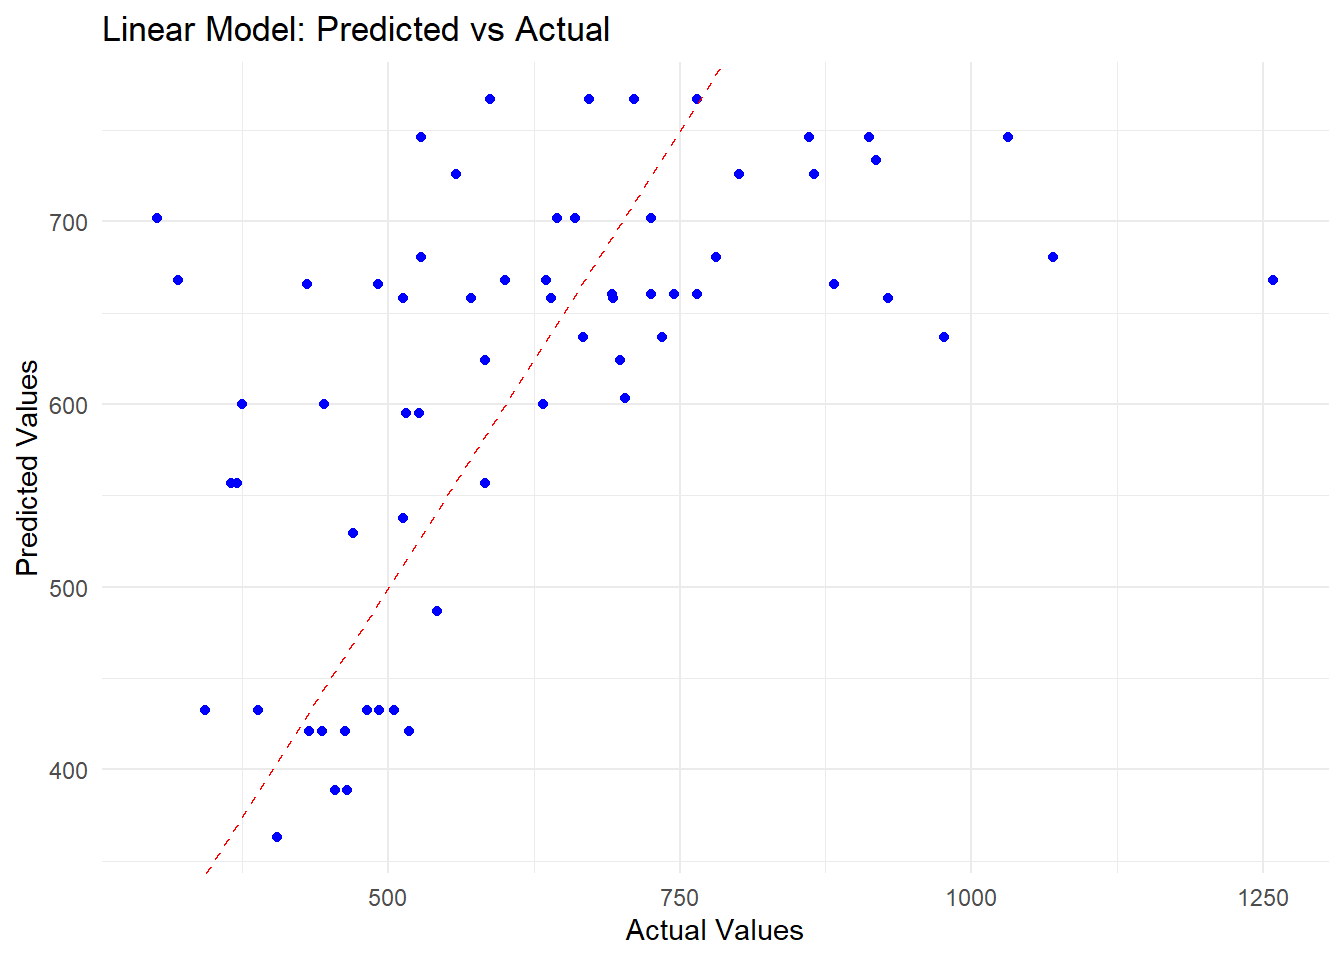
\includegraphics{Updated_Arknights_Operators_Project_Report_files/figure-latex/unnamed-chunk-18-1.pdf}

\section{6. Conclusion}\label{conclusion}

Based on the RMSE results: - \textbf{Random Forest} performed the best
with the lowest RMSE. - \textbf{Lasso Regression} was able to reduce
overfitting and selected important features, with a better performance
than Linear Regression. - \textbf{Linear Regression} performed the
worst, suggesting that the relationships between the predictors and the
outcome are not strictly linear.

Variable importance: - The variable importance chart of Random Forest
shows that base health (base\_hp) and class (class) are important
factors in predicting maximum attack value, especially for certain class
types (such as Defender and Medic).

\begin{itemize}
\tightlist
\item
  In addition, base defense (base\_def) contributes less to predicting
  attack value, but still has some effect.
\end{itemize}

Next, we can further improve the prediction accuracy by further
adjusting the hyperparameters of the random forest model or exploring
other complex nonlinear models (such as support vector machines or
neural networks).

In terms of variable selection, Lasso regression can provide a reference
for future feature selection and model simplification, and further
analyze the important variables selected in the Lasso model.

\end{document}
